\documentclass[11pt,letterpaper]{article}
\usepackage[lmargin=1in,rmargin=1in,tmargin=1in,bmargin=1in]{geometry}
\usepackage{../style/homework}
\usepackage{../style/commands}
\setbool{quotetype}{true} % True: Side; False: Under
\setbool{hideans}{false} % Student: True; Instructor: False

% -------------------
% Content
% -------------------
\begin{document}

\homework{2: Due 09/08}{Money does not buy you happiness, but lack of money certainly buys you misery.}{Daniel Kahneman}

% Problem 1
\problem{10} Suppose that for a certain product, a company has a revenue given by $R(q)= 53.6q$ and costs given by $C(q)= 228 + 23.7q$, where $q$ is thousands of items and $R$, $C$ are measured in tens of thousands of dollars.
	\begin{enumerate}[(a)]
	\item What are the fixed costs? What are the variable costs?
	\item What is the cost production per item? How much would it cost to product 5,200~items?
	\item How much does the product sell for? What is the revenue yielded by selling 2,000~items?
	\item Find the profit function, $P(q)$.
	\item What is the smallest number of individual units of this product the company must sell to make a profit?
	\end{enumerate} \pspace

\sol
\begin{enumerate}[(a)]
\item The fixed costs are the costs when no product is produced, i.e. $C(0)$. But then we have $C(0)= 228 + 23.7(0)= 228 + 0= 228$~tens of thousands of dollars. Therefore, the fixed costs are \$2,280,000. Because $C(q)= 228 + 23.7q$ is a linear cost function, the variable cost is the slope of $C(q)$. The slope of $C(q)$ is 23.7, i.e. the cost of production in tens of thousands of dollars per thousand items. \pspace

\item Because $C(q)= 228 + 23.7q$ is a linear cost function, the variable cost is the slope of $C(q)$. The slope of $C(q)$ is 23.7, i.e. the cost of production per thousand items. The cost of producing 5,200~items, i.e. 5.2~thousand items, is $C(5.2)= 228 + 23.7(5.2)= 228 + 123.24= 351.24$~tens of thousands of dollars, i.e. \$3,512,400.00. \pspace

\item Because $R(q)= 53.6q$ is linear, the slope of $R(q)$ is the price of each product. The slope of $R(q)$ is 53.6; therefore, each thousand items sells for 53.6~tens of thousands of dollars, i.e. \$536 per item. The revenue of selling 2,000~items, i.e. 2.0~thousand items, is $R(2.0)= 53.6(2.0)= 107.2$~tens of thousands of dollars, i.e. \$1,072,000.00. \pspace

\item Profit is the revenue minus the cost, i.e. $P(q)= R(q) - C(q)$. Therefore, we have\dots
	\[
	P(q)= R(q) - C(q)= 53.6q - (228 + 23.7q)= 53.6q - 228 - 23.7q= 29.9q - 228.
	\] \pspace

\item This is the breakeven point, and occurs at a production level where $P(q)= 0$ (equivalently, $R(q)= C(q)$). But if $P(q)= 0$, then we have $29.9q - 228= 0$. But then $29.9q= 228$ so that $q= 7.62542$~thousand items, i.e. 7,625.42 items. Therefore (because 7,625.42 is the number of items to obtain profit zero and selling any less, results in less revenue), they have to sell at least 7,626~items.
\end{enumerate}



\newpage



% Problem 2
\problem{10} Ben and Jerry own an ice cream truck called `The Rolling Cones.' Each day, they drive the truck around the boroughs of NYC trying to satisfy customers in the summer heat. All the standard soft serve flavors sell for the same sale price. Once it is averaged out, the cost of the mixed used to make the cones costs approximately \$0.09 per cone. To turn a profit, they mark-up the cost per cone to \$2.00. However, the cost to run their truck and pay for upkeep, keep their vending license, and pay other associated costs is roughly \$4,235 per month. 
	\begin{enumerate}[(a)]
	\item Find Ben and Jerry's revenue function.
	\item What are Ben and Jerry's variable and fixed costs?
	\item Find Ben and Jerry's cost function. 
	\item What is the minimum number of cones that they must sell each month to turn a profit?
	\end{enumerate} \pspace

\sol
\begin{enumerate}[(a)]
\item The revenue function, $R(q)$, is the amount they make by selling $q$ cones. Because each cone costs \$2.00, by selling $q$ cones, they make $2q$, i.e. $R(q)= 2q$. \pspace

\item The variable costs are the costs of producing $q$ cones. Because each cone costs \$0.09 to produce, by producing $q$ cones, the variable costs are $0.09q$. The fixed costs are the costs they incur regardless the level of production. Because they must pay \$4,235, regardless of the number of cones that they make, their fixed costs are $4235$. \pspace

\item The cost function, $C(q)$, is the cost associated with producing $q$ cones. Because the costs consist of variable and fixed costs, we know that $C(q)= \text{VC} + \text{FC}$. But then by (b), we have $C(q)= 0.09q + 4235$. \pspace

\item Because both $R(q)$ and $C(q)$ are linear, the point at which they start to turn a profit is the equilibrium point, i.e. the level of production $q$ at which $R(q)= C(q)$. But then we have\dots
	\[
	\begin{aligned}
	R(q)&= C(q) \\[0.3cm]
	2q&= 0.09q + 4235 \\[0.3cm]
	1.91q&= 4235 \\[0.3cm]
	q&= 2217.28
	\end{aligned}
	\]
Because $q= 2217.28$ is the minimum number of cones they must produce/sell to have a profit of zero and producing/selling less cones results in less revenue (and hence less profit), they must produce/sell at least 2,218 cones. 
\end{enumerate}



\newpage



% Problem 3
\problem{10} A local radio station charges approximately \$1,800 per advertising slot to local businesses. The building where the radio station is located costs them \$48,000 per month to rent and they pay \$18,360 in electricity each month. Additionally, the cost to pay their employees, cover health insurance, stock the office, purchase and maintain equipment, etc. is approximately \$162,000. Determine the revenue, cost, and profit functions. Then find the equilibrium point. Finally, sketch a plot of all of these in the graph below, being carefully to label your plot and indicate the equilibrium point. \pspace

\sol Because the station charges \$1,8000 per slot, $q$, the revenue function, $R(q)$, is given by $R(q)= 1800q$. The cost associated with offering (producing) and selling $q$ slots, $C(q)$, is the sum of the fixed and variable costs. There are no variable costs (as described) for offering and selling $q$ slots. However, because the station has to rent the building at a cost of \$48,000 per month, pay \$18,360 in electricity per month, and pay their employees, cover health insurance, stock the office, purchase and maintain equipment at a cost of \$162,000 per month, the station's fixed costs are $48000 + 18360 + 162000= 228360$. But then we have $C(q)= \text{VC} + \text{FC}= 0 + 228360= 228360$. The revenue function, $R(q)$, for offering (producing) and selling $q$ advertising slots is $P(q)= R(q) - C(q)= 1800q - 228360$. The equilibrium point is the point at which $R(q)= C(q)$, i.e. the point where $P(q)= 0$. But then we have\dots
	\[
	\begin{aligned}
	1800q - &228360= 0 \\[0.3cm]
	1800q &= 228360 \\[0.3cm]
	q&= 126.867
	\end{aligned}
	\]
Note that we have $R(126.867)= C(126.867)= 228360$, so that the equilibrium point is $(126.867, 228,360)$. We can then plot $R(q)$, $C(q)$, and $P(q)$ on the plot below. [Note that the $x$-axis will be measured in number of advertising slots sold, $q$, and the $y$-axis will be measured in tens of thousands of dollars.]





	\vfill
	\[
	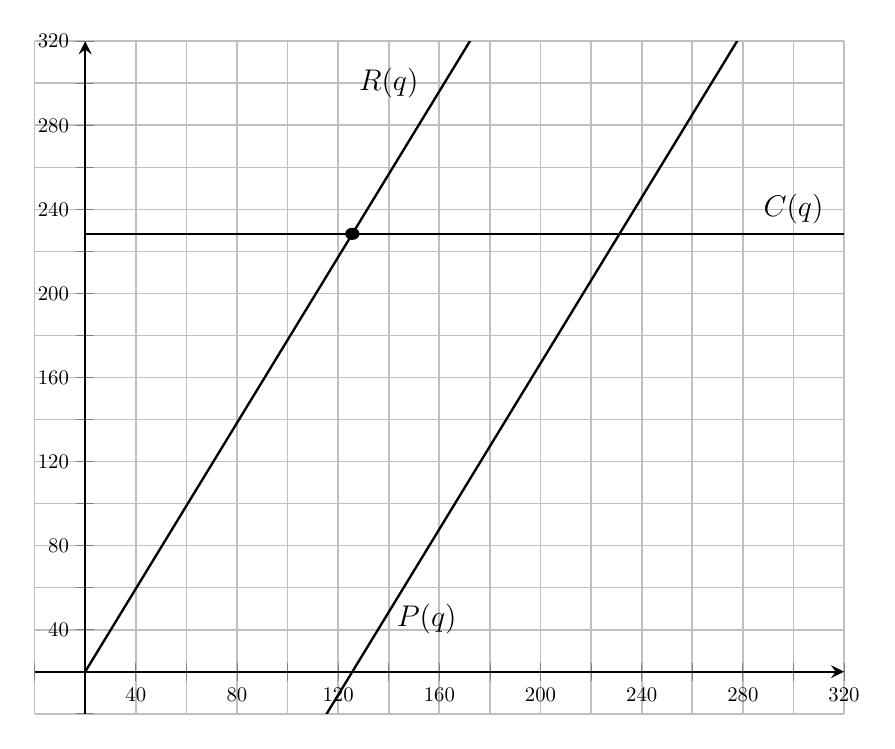
\begin{tikzpicture}[scale=1.5,every node/.style={scale=0.5}]
	\begin{axis}[
	grid=both,
	axis lines=middle,
	%ticklabel style={fill=blue!5!white},
	xmin= -20, xmax=300,
	ymin= -20, ymax=300,
	xtick={-20,0,...,300},
	ytick={-20,0,...,300},
	xticklabels={,,40,,80,,120,,160,,200,,240,,280,,320},
	yticklabels={,,40,,80,,120,,160,,200,,240,,280,,320}
	%xlabel=\(x\),ylabel=\(y\),
	]
	\addplot[line width= 0.02cm,domain= 0:300] ({x},{208.36}); 	
	\addplot[line width= 0.02cm,domain= 0:300] ({x},{1.97278*x}); 
	\addplot[line width= 0.02cm,domain= 0:300] ({x},{1.97278*x - 208.36}); 
	\draw[fill=black] (105.617,208.36) circle (2.5);
	\node at (120,280) {\Large$R(q)$};
	\node at (280,220) {\Large$C(q)$};
	\node at (135,25) {\Large$P(q)$};
	\end{axis}
	\end{tikzpicture}
	\]



\newpage



% Problem 4
\problem{10} Suppose that a company has a revenue function given by $R(q)= 15.8q^2$ and cost function given by $C(q)= 3.1q^2 - 10.8q + 891$, where $q$ is measured in hundreds of items and $R$, $C$ are measured in hundreds of dollars. 
	\begin{enumerate}[(a)]
	\item Find the fixed cost. 
	\item Is the marginal revenue \$15.8 hundreds of dollars per item and the marginal cost \$3.1 hundreds of dollars per item? Explain why or why not. 
	\item Find the average and marginal revenue at a production level of 1,000~items. 
	\item Find the average and marginal cost at a production level of 1,000~items. 
	\item What is the profit at a production level of 1,000~items?
	\end{enumerate} 

\sol
\begin{enumerate}[(a)]
\item The fixed costs are the costs when there are no items produced, i.e. $C(0)$. But then we have $C(0)= 3.1(0) - 10.8(0) + 891= 0 + 0 + 891= 891$~hundreds of dollars, i.e. \$89,100.

\item No. The given revenue and cost functions, $R(q)$ and $C(q)$, respectively, are not linear. Therefore, one cannot simply `read them off' the functions themselves. Furthermore, the marginal revenue and marginal cost are (likely) not constant. 

\item At a production level of 1,000~items, i.e. 10~hundred items, noting that $R(10)= 15.8(10^2)= 1580$ hundreds of dollars, i.e. \$158,000, and $R(11)= 15.8(11^2)= 1911.8$ hundreds of dollars, i.e. \$191,180, we have\dots
	\[
	\begin{aligned}
	\text{Avg. Rev}(10)= \dfrac{R(10)}{10}= \dfrac{1580}{10}= 158 \\[0.3cm]
	\text{Marg. Rev}(10)= \dfrac{R(11) - R(10)}{11 - 10}= \dfrac{1911.8 - 1580}{1}= 331.80
	\end{aligned}
	\] 
Therefore, at a production level of 1,000~items, the average revenue is \$158 hundreds of dollars per thousand items, i.e. \$15.8/item, and the marginal revenue is \$331.80 hundreds of dollar per thousand items, i.e. \$33.18/item.


\item At a production level of 1,000~items, i.e. 10~hundred items, noting that $C(10)= 3.1(10^2) - 10.8(10) + 891=  310 - 108 + 891= \$1093$~hundreds of dollars, i.e. \$109,300, and $C(11)= 3.1(11^2) - 10.8(11) + 891=  375.1 - 118.8 + 891= \$1147.30$~hundreds of dollars, i.e. \$114,730, we have\dots
	\[
	\begin{aligned}
	\text{Avg. Cost}(10)= \dfrac{C(10)}{10}= \dfrac{1093}{10}= 109.3 \\[0.3cm]
	\text{Marg. Cost}(10)= \dfrac{C(11) - C(10)}{11 - 10}= \dfrac{1147.30 - 1093}{1}= 54.3
	\end{aligned}
	\] 
Therefore, at a production level of 1,000~items, the average cost is \$109.3 hundreds of dollars per thousand items, i.e. \$10.93/item, and the marginal cost is \$54.3 hundreds of dollar per thousand items, i.e. \$5.43/item.
 
\item At a production level of 1,000~items, i.e. 10~hundred items, the profit is $P(10)= R(10) - C(10)= \$1580 - \$1093= \$487$~hundreds of dollars per thousands of items, i.e. \$48.7/item.
\end{enumerate}


\end{document}